\begin{figure*}[t]
  \centering
  \begin{subfigure}[b]{0.32\textwidth}
    \centering
    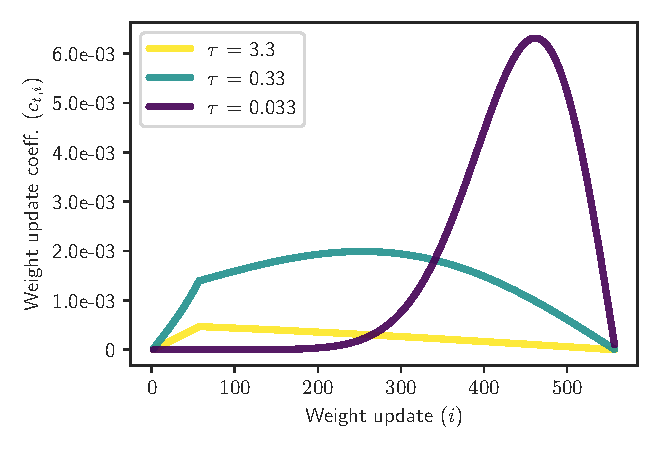
\includegraphics[trim={0.3cm 0.4cm 0.3cm 0.3cm}, clip, width=\linewidth]{pdffigs/111M.tepoch.linear.D2Z.WD=varies.0.2TPP.v2.pdf}
    \label{fig:emas_tepoch_2TPP}
    \caption{557 steps}
  \end{subfigure}
  \hfill
  \begin{subfigure}[b]{0.32\textwidth}
    \centering
    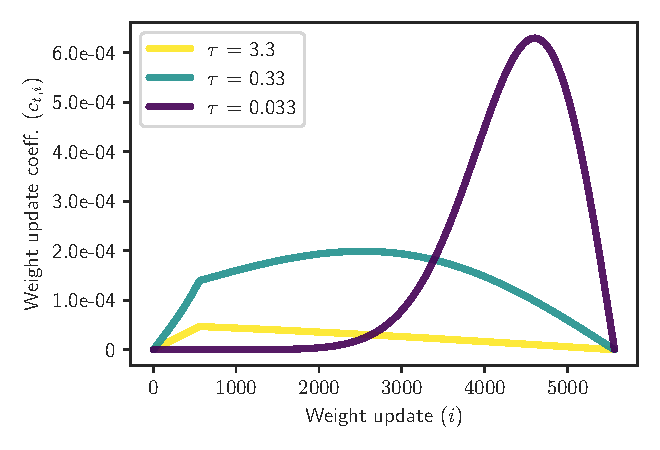
\includegraphics[trim={0.3cm 0.4cm 0.3cm 0.3cm}, clip, width=\linewidth]{pdffigs/111M.tepoch.linear.D2Z.WD=varies.0.20TPP.v2.pdf}
    \label{fig:emas_tepoch_20TPP}
    \caption{5568 steps}
  \end{subfigure}
  \hfill 
  \begin{subfigure}[b]{0.32\textwidth}
    \centering
    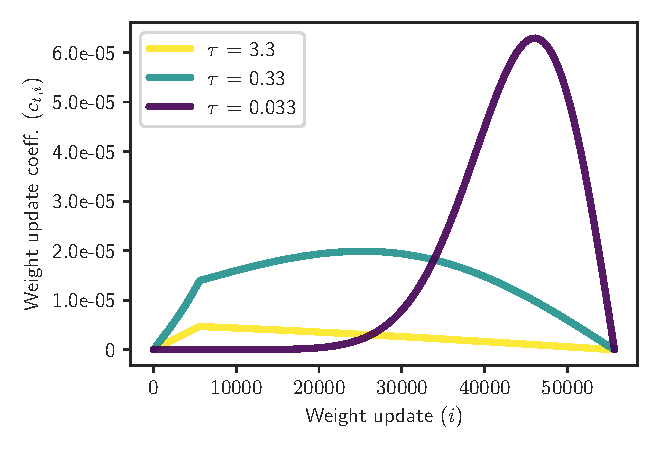
\includegraphics[trim={0.3cm 0.4cm 0.3cm 0.3cm}, clip, width=\linewidth]{pdffigs/111M.tepoch.linear.D2Z.WD=varies.0.200TPP.v2.pdf}
    \label{fig:emas_tepoch_200TPP}
    \caption{55680 steps}
  \end{subfigure}
  \caption{\textbf{$\tepoch$ is invariant to steps, with a learning
      rate decay schedule} (111M scale, proxy-tuned peak $\eta$ with
    linear decay-to-zero): Here we adjust weight decay, $\lambda$, in
    order to maintain $\tepoch$ at a constant value, decreasing
    $\lambda$ proportional to the increase in $S$.  Regardless of the
    total number of optimization steps, we see that the same $\tepoch$
    corresponds to the same \emph{shape} of the distribution of weight
    update coefficients (i.e., the same shape over the \emph{data},
    regardless of how the data is discretized in training).  For batch
    sizing, this means that if we use a constant $D$ but increase $B$
    by $K$$\times$ (decreasing $S$ by $K$$\times$), we will
    incorporate information across the {data} similarly---provided
    we use the same $\tepoch$.\label{fig:emas_tepoch}}
\end{figure*}
